%\documentclass[runningheads,a4paper]{llncs}
\documentclass[10pt,a4paper]{article}
\usepackage[latin1]{inputenc}
\usepackage{amsmath}
\usepackage{amsfonts}
\usepackage{amssymb}
\usepackage{graphicx}
\graphicspath{ {images/} }

\usepackage{wrapfig}

\usepackage[toc,page]{appendix} % enumerating appendixes 
\newcommand{\stoptocwriting}{%
	\addtocontents{toc}{\protect\setcounter{tocdepth}{-5}}}
\newcommand{\resumetocwriting}{%
	\addtocontents{toc}{\protect\setcounter{tocdepth}{\arabic{tocdepth}}}} 

\usepackage{multicol}
\usepackage{geometry,    multirow,   amsthm, url,array}

\usepackage{tabularx}
\usepackage{longtable,booktabs}% my add-on  

\setlength{\parskip}{0.8ex}
\usepackage{xcolor}
\newcommand\myworries[1]{\textcolor{red}{#1}}
% Generated by GrindEQ Word-to-LaTeX 2007 
% LaTeX/AMS-LaTeX

%%% remove comment delimiter ('%') and specify encoding parameter if required,
%%% see TeX documentation for additional info (cp1252-Western,cp1251-Cyrillic)
%\usepackage[cp1252]{inputenc}

%%% remove comment delimiter ('%') and select language if required
%\usepackage[english,spanish]{babel}

%\usepackage{amssymb}
%\usepackage{amsmath}

%%% remove comment delimiter ('%') and select graphics package
%%% for DVI output:
%\usepackage[dvips]{graphicx}
%%% or for PDF output:
%\usepackage[pdftex]{graphicx}
%%% or for old LaTeX compilers:
%\usepackage[dvips]{graphics}


\usepackage{colortbl}
\usepackage{xcolor}

\newlength\mylength
\newcolumntype{C}[1]{>{\centering\arraybackslash}p{#1}} % centering cels in longtables

\usepackage{chngcntr} % number of sections include ssections
\counterwithin{table}{section}% table  include number of sectionn
\counterwithin{figure}{section}% figure   include number of section

\numberwithin{equation}{section} % equation   include number of section

% bibliography
\usepackage{biblatex} %Imports biblatex package
\addbibresource{references.bib} %Import the bibliography file

%charts
\usepackage{pgfplots}
% end charts

%breake url lines in bibliography
\usepackage{url}
\usepackage{breakurl} 
\usepackage[breaklinks]{hyperref}
%end  breake url lines in bibliography

%Theorem-like
% Загрузка пакет hyperref
\usepackage{hyperref}
\hypersetup{
	colorlinks=true, %set true if you want colored links
	linktoc=all,     %set to all if you want both sections and subsections linked
	% % %     linkcolor=blue,  %choose some color if you want links to tand out
	linkcolor=blue,
	filecolor=magenta,      
	urlcolor=cyan,
}
\usepackage{enumitem}
\makeatletter
\def\namedlabel#1#2{\begingroup
	#2%
	\def\@currentlabel{#2}%
	\phantomsection\label{#1}\endgroup
}
\makeatother
\theoremstyle{plain}
\newtheorem{thm}{Theorem}[section]
\newtheorem{lem}[thm]{Lemma}
\newtheorem{prop}[thm]{Proposition}
\newtheorem{cor}{Corollary}[section]

\theoremstyle{definition}
\newtheorem{defn}{Definition}[subsection]
\newtheorem{conj}{Conjecture}[section]
\newtheorem{exmp}{Example}[section]

\theoremstyle{remark}
\newtheorem*{rem}{Remark}
\newtheorem{note}{Note}[section]
% end Theorem-like

% Переносы математики.
\begingroup
\catcode`\+\active\gdef+{\mathchar8235\nobreak\discretionary{}{\usefont{OT1}{cmr}{m}{n}\char43}{}}
\catcode`\-\active\gdef-{\mathchar8704\nobreak\discretionary{}{\usefont{OMS}{cmsy}{m}{n}\char0}{}}
\catcode`\=\active\gdef={\mathchar12349\nobreak\discretionary{}{\usefont{OT1}{cmr}{m}{n}\char61}{}}
\catcode`\<\active\gdef<{\mathchar"313C\nobreak\discretionary{}{\usefont{OML}{cmm}{m}{n}\char60}{}}
\catcode`\>\active\gdef>{\mathchar"313E\nobreak\discretionary{}{\usefont{OML}{cmm}{m}{n}\char62}{}}
\endgroup
\def\times{\mathchar8706\nobreak\discretionary{}{\usefont{OMS}{cmsy}{m}{n}\char2}{}}
\def\subset{\mathchar"321A\nobreak\discretionary{}{\usefont{OMS}{cmsy}{m}{n}\char26}{}}
%\supset,\subseteq,\notin
\def\supset{\mathchar"321B\nobreak\discretionary{}{\usefont{OMS}{cmsy}{m}{n}\char27}{}}
\def\subseteq{\mathchar"3212\nobreak\discretionary{}{\usefont{OMS}{cmsy}{m}{n}\char18}{}}
\def\neq{\not=\nobreak\discretionary{}{\usefont{OMS}{cmsy}{m}{n}\char54\usefont{OT1}{cmr}{m}{n}\char61}{}}
\def\sim{\mathchar"3218\nobreak\discretionary{}{\usefont{OMS}{cmsy}{m}{n}\char24}{}}
\def\in{\mathchar"3232\nobreak\discretionary{}{\usefont{OMS}{cmsy}{m}{n}\char50}{}}
\def\to{\mathchar"3221\nobreak\discretionary{}{\usefont{OMS}{cmsy}{m}{n}\char33}{}}
\def\?#1{#1\nobreak\discretionary{}{\hbox{$\mathsurround=0pt #1$}}{}}
% Конец переносов математики.


\date{}
\raggedbottom
\begin{document}
	\begin{figure}[htbp]
	%[trim=2cm 24.2cm 13.1cm 2.2cm, clip=true, totalheight=0.105\textheight, angle=0]
		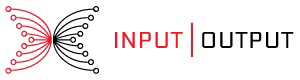
\includegraphics  {iohk-share-logo.jpg}
	\end{figure}
	
	\leavevmode \\ 
	{\Large\textbf{ Comparison of Block Expectation Time for Various Consensus Algorithms }}\\[0,5cm]
	\hrule height 0,1cm \leavevmode \\ 
	
	%	\skip
	\leavevmode \\ 
	{	\small{March 22 \textsuperscript{nd} 2017}}\\ 
	\leavevmode \\ 
	
	\begin{figure}[htbp]
		
		\begin{subfigure} %{0.3\textwidth}
			
	%		\includegraphics [scale=0.3]{etc2.png}
		\end{subfigure}
		\hfill
		\begin{subfigure} %{0.3\textwidth}
	%		\includegraphics [scale=0.2]{creative_commons.jpg}
		\end{subfigure}
	\end{figure}
	
	%	\leavevmode \\[0,5cm] 
	%{\textbf{The Veritas Team}}\\[0,5cm]
	%\leavevmode \\[0,5cm]
	
	%	\skip
	
	\leavevmode \\[0,5cm] 
	{\textbf{The Veritas Team}\\ 
		\\ 
		Dmytro Kaidalov, Lyudmila Kovalchuk, Andrii Nastenko,\\ Mariia Rodinko, Oleksiy Shevtsov, Roman Oliynykov
		\\  
		\\ IOHK.io }\\[0,5cm]
	\leavevmode \\[0,5cm]
	%	\skip
	
	
	%\maketitle
	
	%	\skip
	
	\begin{abstract}
	The blockchain technology emerged in 2008 with Bitcoin appearance. Its main technical innovation is a decentralized consensus mechanism that allows to maintain an uncensored public ledger of transactions hence giving users security guarantees that the data in a ledger can not be modified or reverted in any way. In this paper we examine typical double-spend attacks on the different blockchain-based systems and compare resulting probabilities of success for each of them. In our research we considered classical Bitcoin-like proof-of-work protocol, the GHOST protocol and recently introduced proof-of-stake algorithm called Ouroboros.
	\end{abstract}
	
	
	\begin{flushleft}
		\eject 
		
	\end{flushleft}
	
	
	\tableofcontents
	
	\begin{flushleft}
		\eject 
		
	\end{flushleft}
	
	\section{Introduction}
	The Bitcoin is a payment system where digitally signed transactions are grouped into blocks and stored securely in a structure called blockchain. A blockchain is a sequence of blocks linked via hash pointers where each new block contains a hash of the previous block. This structure preserves an ordered list of transactions that uniquely determines state of the system.
	
	Unlike other centralized payment systems, in Bitcoin, once a transaction is added to the blockchain it could not be considered as confirmed immediately. A user need to wait some time to be sure that the transaction is set in stone in the blockchain. This is because of decentralized nature of the system where everyone can add blocks to the blockchain. To guarantee consistency among different users and to preserve inability to revert previously added blocks, a special mechanism is used called proof-of-work. The following idea underlies a proof-of-work system: a computational effort (calculation of a hash value below some target) should be spend to produce a block. Only a chain of blocks with the most computations is considered valid.
	
	As the blockchain technology evolves the alternatives to the computationally heavy proof-of-work mechanism appear. The one most promising is called proof-of-stake: it does not require heavy computations to produce blocks, instead, a block producer is chosen through a fair procedure among all stakeholders in the system. The Ouroboros, claimed by the authors as the first provably secure proof-of-stake protocol, is a good example of such a system.
	
	The concept of a blockchain could be undermined if someone would have a possibility to revert blocks by submitting a chain with more computations in it. For example, it could lead to the following attack: some buyer pays to a merchant with bitcoins, after the corresponding transaction is included into the blockchain the merchant accepts a payment and sends a product to the buyer, upon receiving the product the buyer issues a conflicting chain of blocks which does not contain the payment to the merchant but instead sends coins to the buyer. As long as a recipient could not be sure that a payment is irreversible it is insecure to deliver a product.
	
	Satoshi Nakomoto argues in the original Bitcoin white paper \cite{N08} that the system is secure (with some probability) against such attacks unless more than 50\% of the computational power possessed by an attacker.
	
	The described double-spend attack is relevant not only for Bitcoin, but also for other proof-of-work systems, for instance, those based on GHOST algorithm [?], as well as for proof-of-stake systems, like Ouroboros. In this paper we compare different consensus protocols, as a measure we focus on the block confirmation time needed to provide reasonable security guarantees for the users. 
	
	The paper is structured in the following way: the second chapter describes classical double-spend attack for Bitcoin as it was introduced by S. Nakomoto. The third chapter describes splitting attacks that are relevant to those proof-of-work systems where the time difference between blocks is not negligible compared to the block propagation time. The fourth chapter describes a double-spend attack for Ouroboros proof-of-stake protocol. The last chapter summarizes and compares results from the previous chapters. 
	 
	
	\section{Double-Spend Attack: General Overview} \label{double-spend-attack-general-overview}
	
	This section represents an overview of how a double-spend attack could happen in a blockchain-based system. As we briefly mentioned before it does not really matter what type of consensus mechanism underlies the system, a double-spend could happen in both proof-of-work and proof-of-stake system. An interested reader could find more information in \cite{bitcoinwiki}.
	
	As it follows from the name, the whole idea of a double-spend attack is to use the same coins twice. Usually it implies that someone pays for some goods, but after receiving it reverts the payment so both goods and money are in the hands of an attacker. While it is infeasible to change the transaction with the payment itself (cause that would require falsifying a digital signature) it is possible to reject an entire block which includes the transaction. For doing this an attacker needs to substitute a valid sub-chain of blocks with a new one that has a bigger score (score computation depends on the actual blockchain type). Even though this attack requires tremendous resources (computational in the case of proof-of-work or stake in the case of proof-of-stake system) it could be profitable.
	
	The attack involves next steps:
	\begin{enumerate}
        \item An attacker A wants to buy some goods from a merchant B. For this, A creates a transaction \(tx_1\) with payment to B and sends it to the blockchain (Fig. \ref{fig:Fig1}).
        \item B receives the payment from A, he waits suitable number of confirmations in the blockchain and then sends goods to the A (Fig. \ref{fig:Fig2}).
        \item A creates a conflicting transaction \(tx_2\) where he redirects coins to his adderess and tries to generate a forked block containing this transaction. Given that B waits additional confirmations on top of the block with the payment, A needs to overcome all those blocks in the main chain and create a fork with a higher score (Fig. \ref{fig:Fig3}).
        \item If A is lucky to produce a fork of the main chain the transaction \(tx_1\) would be removed from the blockchain. Instead, the transaction \(tx_2\) would be included. The network will continue with the chain of the attacker so the payment for the merchant B would be lost forever (Fig. \ref{fig:Fig4}). At the same time the attacker A seizes both goods and money.
    \end{enumerate}
    
    \begin{figure}[h]
            \centering
            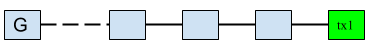
\includegraphics[width=0.4\textwidth]{Fig1}
            \caption{Initial state of the blockchain from the genesis block G. The transaction \(tx_1\) is just included in the last block.}
            \label{fig:Fig1}
    \end{figure}
    \begin{figure}[h]
            \centering
            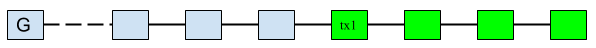
\includegraphics[width=0.6\textwidth]{Fig2}
            \caption{Merchant B waits for 3 more blocks on top of the block with \(tx_1\) and sends goods to A.}
            \label{fig:Fig2}
    \end{figure}
    \begin{figure}[h]
            \centering
            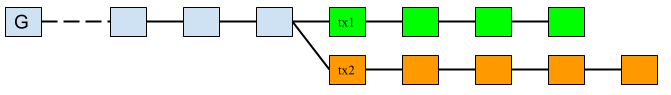
\includegraphics[width=0.7\textwidth]{Fig3}
            \caption{An attacker creates a fork}
            \label{fig:Fig3}
    \end{figure}
    \begin{figure}[h]
            \centering
            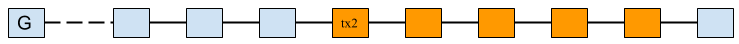
\includegraphics[width=0.78\textwidth]{Fig4}
            \caption{A network continues with the chain of the attacker}
            \label{fig:Fig4}
    \end{figure}
    
    Even though an exact techniques of a fork creation could varies for different consensus protocols, the essence of the described attack remains the same for all of them. 
	
	\section{Bitcoin Double-Spend Attack}
	
	This section represents different mathematical models of the double-spend attack for Bitcoin protocol. The first one was introduced by S. Nakomoto in the original Bitcoin white paper [?]. M. Rosenfeld continued research of the Nakomoto's model and improved it in [?]. We also describe two models proposed by C. Pinzon et al. that introduced a notion of time advantage to the original model that was analyzed by Nakomoto and Rosenfeld.
	
	\subsection{The Model of S. Nakomoto}
	
	S. Nakomoto considers the scenario when an attacker tries to generate secretly an alternate chain that would be longer (in terms of computational difficulty) than the honest chain. The race between the attackers chain and the honest chain is characterized as Binomial Random Walk.
	
	Given that an attacker starts with some deficit \(K\) (the honest chain is longer than the attacker`s chain on \(K\) blocks), the probability that an attacker would ever catching up with the honest chain is analagous to the Gambler's Ruin problem and could be calculated as follows:
	\[ q_z = 
	    \left \{
            \begin{tabular}{cc}
                1       & \(if\  p \leq q\) \\
                \((q/p)^z\) & \(if\  p > q\) \\
            \end{tabular}
        \right \},
	\]
	where
	
	\(p\) - fraction of hashing power that is possessed by honest nodes (equivalent to the probability that an honest node finds next block);
	
	\(q\) - fraction of hashing power that is possessed by attacker (equivalent to the probability that an attacker finds next block);
	
	\(q_z\) - probability that an attacker would ever catch up from the deficit of \(K\) blocks.
	
	Assuming that an attacker starts to work on malicious fork right after the payment transaction is included into the blockchain (so do not wait for \(z\) blocks after which it is confirmed by the merchant), he may have mined some number of blocks so the deficit \(K\) is reduced. The attackers progress will be a Poisson distribution with expected value \( \lambda = z\frac{q}{p} \).
	
	Now to get overall probability of the successful double-spend attack we need to multiply the Poisson density for each possible amount of progress of an attacker by the probability he would catch up from the remaining deficit:
	\begin{equation} \label{eq:nak_DS}
	    DS_N(q,z) =
	    \sum_{k=0}^{\infty} \frac{\lambda^k e^{-\lambda}}{k!} \cdot
	    \left \{
            \begin{tabular}{cc}
                \((q/p)^{z-k}\) & \(if\  k \leq z\) \\
                1       & \(if\  k > z\) \\
            \end{tabular}
        \right \}
        =
        1 - \sum_{k=0}^{z} \frac{\lambda^k e^{-\lambda}}{k!}(1 - (q/p)^{z-k}).
	\end{equation}
	
	More detailed explanation of this model could be found in the original paper [?]. 
	
	\subsection{The Model of M. Rosenfeld}
	
	M. Rosenfeld in his paper \cite{R14} clarify and expand the work of S. Nakomoto. The same basic model is taken: for a successful double-spend attack an attacker needs to catch up from \(z\) blocks where \(z = n - m\) (n - number of blocks in the honest chain, m - number of blocks in attackers chain). 
	
	The aurhor considers the catching-up process as a Markov chain, where each step is defined as finding a block by the honest node or attacker:
	\[ z_{i+1} = 
	    \left \{
            \begin{tabular}{cc}
                z_i + 1 & with probability p \\
                z_i - 1 & with probability q \\
            \end{tabular}
        \right \)
	\]
	
	The attack succeeds if \(z\) ever reaches \(-1\). Let denote by \(\alpha_z\) the probability that an attacker would be able to catch up when he is \(z\) blocks behind. If \(z < 0\) then \(\alpha_z = 1\), otherwise \[\alpha_z = p\alpha_{z+1} + q\alpha_{z-1},\] where \(q\) is a fraction of hashing power possessed by attacker (equivalent to the probability that an attacker finds next block) and \(p = 1 - q\).
	
	In this case the probability of catching up with \(z\) blocks could be calculated as follows:
	\begin{equation}  \label{eq:ros_catchup} 
	    \alpha_z = min(q/p,1)^{max(z+1,0)} = 
	    \left \{
            \begin{tabular}{cc}
                1       & \(if\  z < 0\ or\ q > p\) \\
                \((q/p)^{z+1}\) & \(if\ z \geq 0\ and\ q \leq p\) \\
            \end{tabular}
        \right \) 
	\end{equation}
	
	Similar to the model of S. Nakomoto it is possible that an attacker mined some number of blocks while the merchant waits for \(n\) confirmations in the honest chain. Recall that S. Nakomoto considers the progress of an attacker in this case as a Poisson distribution with expected value \(n\frac{q}{p}\). M. Rosenfeld took another assumption, he model the progress of an attacker as a negative binomial distribution. The probability that an attacker would mine a given number of blocks \(m\) is 
	\begin{equation} \label{eq:ros_progress}
	    P(m) = \binom{m+n-1}{m}p^n q^m. 
	\end{equation}
	
	It follows that the probability of a successful double-spend attack where a merchant waits for \(n\) confirmations and an attacker succeeds to find \(m+1\) blocks during the confirmation period is equal to
	\begin{equation}  \label{eq:ros_DS}
	    DS_R(q,n) = \sum_{m=0}^{\infty}P(m)\alpha_{n-m-1} = 
	    \left \{
            \begin{tabular}{cc}
                1 - \sum_{m=0}^{n}\binom{m+n-1}{m}(p^n q^m - p^m q^n)   & \(if\  q < p\) \\
                1 & \(if\  q \geq p\) \\
            \end{tabular}
        \right \)
	\end{equation}
	
	An interested reader could find a rigorous description of this model in the original paper [?].
	
	\subsection{The Generalized Model of C. Pinzon et al.}
	
	The model proposed by C. Pinzon et al. \cite{PR16} generalizes the model of M. Rosenfeld by adding an extra parameter that represents time-advantage of an attacker.
	
	As in previous models, a successful double-spend attack consists of two constituents: the progress of an attacker during the confirmation period of \(m\) blocks and his ability to catch up from the deficit \(z = m - n\). The catch-up function is the same as originally proposed by S. Nakomoto. The improvement of this model lies in the modified progress function. It could be represented as follows: \[P(q,m,n,t),\] where
	
	\(q\) - fraction of hashing power that is possessed by attacker (equivalent to the probability that an attacker finds next block);
	
	\(m\) - number of blocks in the honest chain;
	
	\(n\) - number of blocks in the malicious chain;
	
	\(t\) - time advantage of an attacker towards fraudulent block production.
	
	Basically the function \(P\) represents the probability of an attacker mining exactly \(n\) blocks once the honest network mines \(m\) blocks assuming that an attacker has been additionally mining secretly for \(t\) time units. While the first three parameters \((q,m,n)\) are well-known from the previous models, the time-advantage \(t\) is the new one. It represents an amount of time since the \(n^{th}\) block is found by an attacker until the \(m^{th}\) block is found by the honest network. This time period \(t\) potentially increases the probability of an attacker to find next block faster than the honest network thus giving him an advantage.
	
	In order to define the function \(P\), it is necessary to define the function \(a(q,t,k)\) that represents the probability to mine exactly \(k\) blocks during the time period \(t\) with a proportion \(q\) of hashing power (the proof could be found in the original paper []):
	\[a(q,t,k) =
	    \left\{
            \begin{array}{11}
                1 & if\  t = n = 0 \\
                0 & if\  t \leq 0 \\
                \frac{(qt)^k}{k!}e^{-qt} & otherwise. \\
            \end{array}
        \right.
	\]
	
	The function \(P\) can be defined as follows:
	\begin{equation}  \label{eq:pin_G_prog}
	    P(q,m,n,t) = \sum_{z=0}^{n}a(q,t,z)P_R(q,m,n-z).
	\end{equation}
	
	Note that in case of \(t=0\) the progress function \(P(q,m,n,t)\) is equivalent to the progress function presented by M. Rosenfeld.
	
	It follows that the probability of a successful double-spend attack is equal to:
	\begin{equation}  \label{eq:pin_G_DS}
	    DS_G(q,K,n,t) = 1 - \sum_{z=0}^{K-n}P(q,K,z,t)(1 - C_R(q,K-n-z)),
	\end{equation}
	where
	
	\(q\) - fraction of hashing power that is possessed by attacker (equivalent to the probability that an attacker finds next block);
	
	\(K\) - number of blocks in the honest chain;
	
	\(n\) - number of blocks in the malicious chain;
	
	\(t\) - time advantage of an attacker;
	
	\(C_R(x,y)\) - catch-up function as defined by M. Rosenfeld (eq. \ref{eq:ros_catchup}).
	
	Note that the functions \(DS_N\) (eq. \ref{eq:nak_DS}) and \(DS_R\) (eq. \ref{eq:ros_DS}) are equevalent to the \(DS_G\) with parameters \(t=0\) and \(n=1\). More information regarding this model could be found in the original paper [?]. 
	
	\subsection{The Time-based Model of C. Pinzon et al.}
	
	The second model presented by C. Pinzon et al. is completely different from those described in the previous sections. In the time-based model the length of the valid and fraudulent chains are assumed to be equal. Instead, authors are focused on the time parameter \(t\) that represents time difference between the \(n^th\) block of both an attacker and honest network.
	
	We will not go deep into the details of this model, instead we will only present the final equation for calculating the probability of a double-spend attack. We refer an interested reader to the original paper [?] to find more details about this model.
	
	The double-spend attack probability can be defined as the probability of having a time disadvantage \(t\) once the \(K+1'th\) block is mined multiplied by the probability of catching up from that disadvantage:
	\begin{equation}  \label{eq:pin_T_DS}
	    DS_T(q,K,n_0,t_0) = \int_{-\infty}^{\infty} P(q,K+1,K-n_0+1,t)C_T(q,t-t_0)dt,
	\end{equation}
	where
	
	\(P\) - progress function from the generalized model (eq. \ref{eq:pin_G_prog});
	
	\(C_T\) - catch up function for the time-based model that is defined as follows:
	\[C_T(q,t) =
	    \left\{
            \begin{array}{11}
                \frac{q}{p}e^{-(p-q)t} & if\ t > 0 \\
                1 & otherwise. \\
            \end{array}
        \right.
	\]
	
	The parameters of the \(DS_T\) are similar to \(DS_G\).
	
	\subsection{Models Comparison}
	
	In this section we compare experimental results obtained with the presented models. Since all considered models are aimed to estimate the probability of the same double-spend attack in Bitcoin, the results are similar except minor difference between the model of S. Nakomoto and others. The models of M. Rosenfeld and C. Pinzon et al. give exactly similar results (assuming that the time advantage in the models of C. Pinzon is equal to zero).
	
	In order to show the numerical values of the probabilities we took data that was presented in [?]. Fig. \ref{fig:Pinzon1} and Table \ref{fig:Pinzon2} represent probabilities of attack for different parameters and models.
	\begin{figure}[]
            \centering
            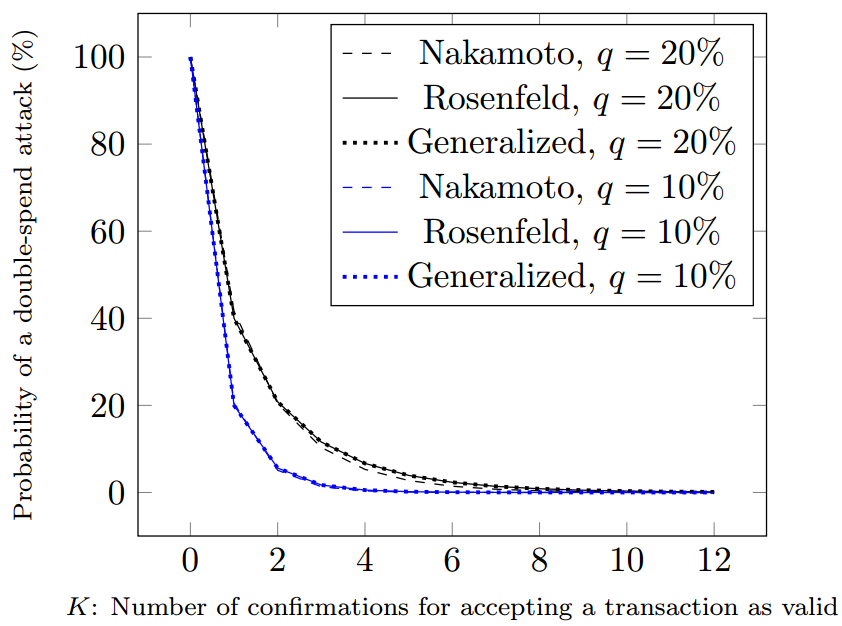
\includegraphics[width=0.75\textwidth]{Pinzon1}
            \caption{Probability of a double-spend attack after \(K\) confirmations}
            \label{fig:Pinzon1}
    \end{figure}
    \begin{table}[]
            \centering
            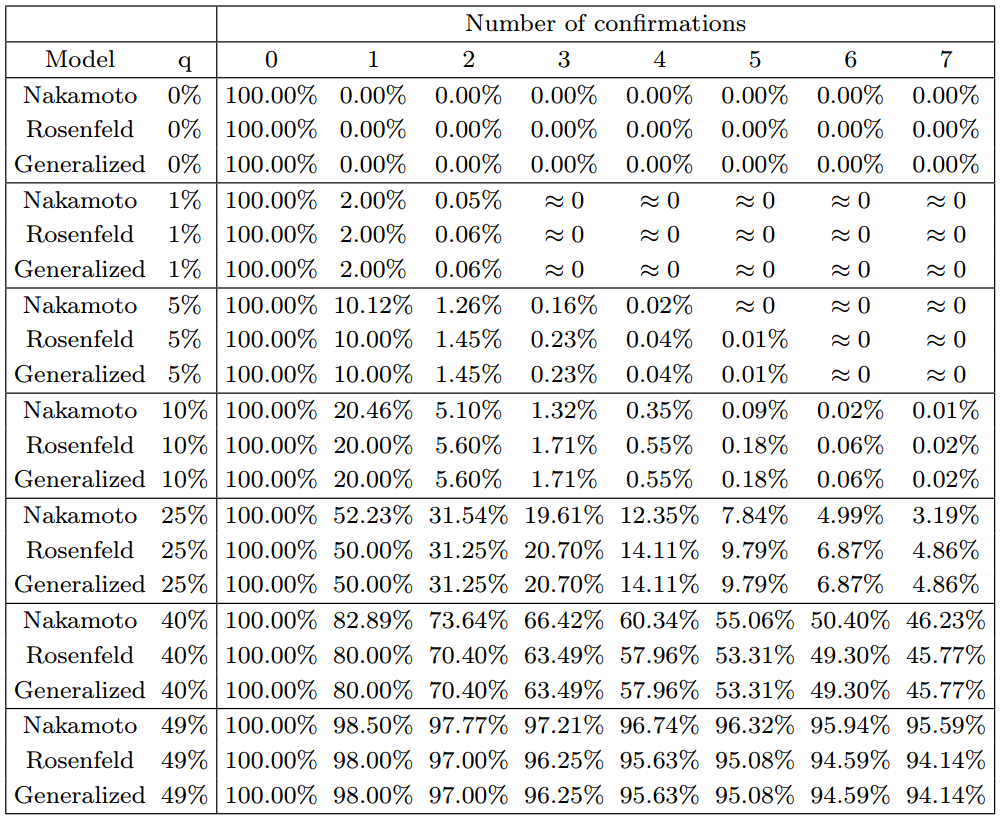
\includegraphics[width=0.85\textwidth]{Pinzon2}
            \caption{Probability of a double-spend attack}
            \label{fig:Pinzon2}
    \end{table}
	
	As we have seen the probability of a double-spend attack drops exponentially with the number of confirmations. Assuming that an attacker possesses 10\% of the total network hash power it is needed to wait for 6 confirmations to be sure that the probability of an attack does not exceed 0.1\%. 
	
	\section{Blockchain Splitting Attacks}
	
	This section provides a description of a splitting attack as it is introduced in \cite{KP15}. It could be considered as a variation of a double-spend attack since the main goal is to create a fork of the required length. The splitting attack is targeted on the proof-of-work based protocols with a short block generation time that is comparable to the block propagation time in the network.
	
	We will start with a general overview of a splitting attack and then provide some experimental results showing the possibility of its application to different proof-of-work consensus protocols.  
	
	\subsection{Splitting Attack: General Overview}
	
	In contrast to classic double-spend attack described in section \ref{double-spend-attack-general-overview} where an attacker is supposed to create a fork secretly and publish it only when it is needed, the splitting attack is public for all nodes from the beginning. Moreover, not only an attacker is supposed to contribute blocks into the forked branch but also honest nodes.
	
	The idea of the attack is the following: when a fork of depth 1 accidentally happens, an adversary splits its hashing power on both branches to keep their lengths\footnotemark \ equal as long as possible. In this case honest miners would also be split due to their arbitrary chose between branches of equal lengths. When honest miners publish a new block on the one of the branches, an adversary publishes block on the other branch to keep the fork running (see Fig. \ref{fig:split}). If branches are of the same length, then adversary does nothing so again honest miners are split in half.
	
	\footnotetext{In most proof-of-work protocols the actual criterion for branch selection is the branch difficulty, i.e., the winning branch is the one that required the most computations to create. For simplicity and because it is usually the case in a real world, it is assumed that all blocks have the same difficulty so the longest chain would be the most difficult one.}
	
	\begin{figure}[h]
            \centering
            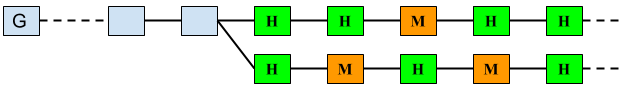
\includegraphics[width=0.75\textwidth]{split}
            \caption{The fork that keeps running while at attacker is able to equalize the lengths of both branches with malicious blocks (marked with M).}
            \label{fig:split}
    \end{figure}
	
	So adversary tries to keep both chains balanced by their length. If lengths differs, adversary extends the chain, that is behind, by publishing some amount of blocks needed to equalize lengths of both chains. The attack continues till adversary has sufficient amount of blocks for each chain in his reserves. If he can't equalize chains lengths at the end of some round, then the attack is finished.
	
	A notion of a round was initially taken from \cite{GKL15}, it represents a complete round of information propagation to all nodes in a p2p network. In practice information propagation is a random variable with an order of tens of seconds. In the described model it is assumed that one full communication round takes 12.6 seconds (this is the average block propagation time in Bitcoin network \cite{DW13}).
	
	A general essence of the splitting attack is the following: when the time of block generation is comparable to the time of block propagation then the probability of generation 2 or more blocks in the same round (and at the same block height) becomes non-negligible. In this case, at the beginning of the next round the network would be split into two branches. An adversary leverages such block collisions to keep the fork running.
	
	Thus, an important parameter that facilitates a splitting attack is the number of POW solutions (mined blocks) per complete round of information propagation. In \cite{KP15}, where this parameter is designated as \(f\), it was shown that when \(f\) decreases and gets closer to 0, then the probability of a splitting attack decreases too (an adversary needs almost 50\% of the hashing power to make a split). And vice versa, when \(f\) increases, the security bound becomes worse (the attack becomes feasible with less than 50\% of the hashing power). The splitting attack is the most effective when \(f \geq 1 \), i.e., at the rate of 1 block per round or more.

    It follows that a short block generation time (relative to the block propagation time) creates favorable conditions for a splitting attack to occur. Hence, it becomes interesting to investigate resistance of Bitcoin-like and GHOST proof-of-work protocols with different values of the parameter \(f\) to the described attack. Further sections represent experimental results obtained during the computational modeling for both protocols.
	
	\subsection{Bitcoin Proof-Of-Work Protocol}
	
	As it is known, the average block generation time in Bitcoin is equal to 10 minutes \cite{N08}. Given that the average block propagation time is 12.6 seconds \cite{DW13}, the parameter \(f=\frac{12.6}{10*60}=0.021\). In what follows it is more suitable to use the parameter \(k\) instead of \(f\) that shows an average amount of communication rounds between 2 consecutive blocks: \(k=\frac{1}{f}\).
	It is interesting to estimate the possibility of a successful splitting attack for the original chose made in Bitcoin where \(k=47.6\). It is also interesting to see how the security degrades in the case when \(k\) decreases. To accomplish this we do an experimental analysis on the described attack. A simulation is done using the Alghorithm \ref{Algo1}.
	
	The results are summarized in Fig. \ref{fig:btc_split_chart}. It is shown what fork length an adversary could maintain with the probability of success at least 1\%. It is easy to see that when the time between blocks decreases an adversary gets a chance to create longer fork. 
	
	Our simulation shows that for the chose of \(k=47.6\) (like in Bitcoin) 6 confirmations are needed to be sure that the probability of a splitting attack is less than 1\% (considering an adversary which possesses 35\% of the hashing power). If we assume that the average block generation time is equal to the block propagation time (so that \(k=1\)) then 9 confirmation is needed for the same level of security.   
	
	\begin{figure}[h]
        \centering
        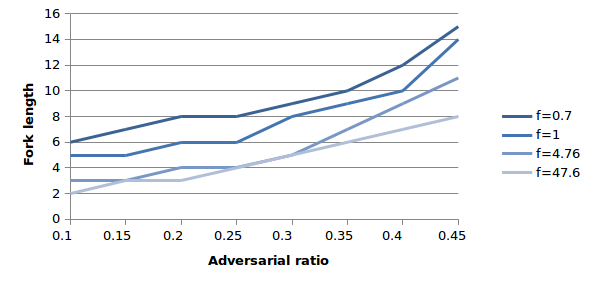
\includegraphics[width=0.75\textwidth]{btc_split_chart}
        \caption{The fork length that an attacker with a given hashing power could create with the probability of success at least 1\%. Different lines represents different chose of the parameter \(k\).}
        \label{fig:btc_split_chart}
    \end{figure}
	
	
	\subsection{GHOST Proof-Of-Work Protocol}
	
    The GHOST (Greedy Heaviest-Observed Sub-Tree) protocol was initially proposed as an improvement of the Bitcoin protocol that allows to reduce the time between blocks while preserving the same level of security \cite{ZS13, ZS15}.
    
    The main modification that was suggested is that blocks that are not included in the main chain can still contribute to a chain's irreversibility. The basic observation behind the protocol is that the blocks that are built on top of some block \(B\) add additional weight to block \(B\) even if they are not in the main chain. So, in contrast to the Bitcoin protocol, where only the blocks that are in the main chain contributes to the difficulty of this chain, in GHOST a whole sub-tree of blocks is considered (Fig. \ref{fig:btc_vs_ghost}). More information in \cite{ZS13,ZS15}.
    
    \begin{figure}[]
        \centering
        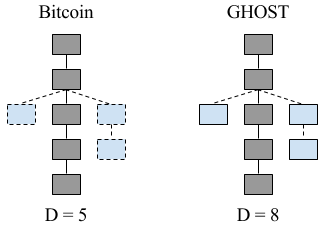
\includegraphics[width=0.4\textwidth]{btc_vs_ghost}
        \caption{The chain's difficulty (D) 7 calculation is shown for the Bitcoin protocol and GHOST protocol. As it could be seen, in GHOST, even the blocks that are not included in the main chain add weight to it.}
        \label{fig:btc_vs_ghost}
    \end{figure}
	
	Since it is declared by the authors that the GHOST protocol has a comparable security even with short block generation time (it is stated that even when blocks are issued every second the security level is the same as in original Bitcoin protocol \cite{ZS13}), it becomes interesting to investigate resistance of the GHOST protocol against splitting attack.
	
	The splitting attack for the GHOST protocol is slightly different compared to Bitcoin \cite{KP15}. There are two differences:
	\begin{enumerate}
    	\item An adversary has to compensate the difference in the total number of honestly mined blocks on both branches at the end of each round, while in Bitcoin-like protocols she has to compensate only the maximal number of honestly mined blocks to keep both chains balanced.
    	\item All blocks produced by an adversary are always valid. This facilitates an attack for adversary, because he can just mine the first nodes after the common prefix of the two branches. In contrast, in Bitcoin an adversary has to extend only the head of diverging chains, so all blocks must be recent. 
	\end{enumerate}
	
	The simulation of the splitting attack for the GHOST protocol was done using the algorithm \ref{Algo2}. The results (Fig. \ref{fig:ghost_split_chart}) show that the attack is extremely effective when the parameter \(k\) is near to 1.
	
	\begin{figure}[h] 
        \centering
        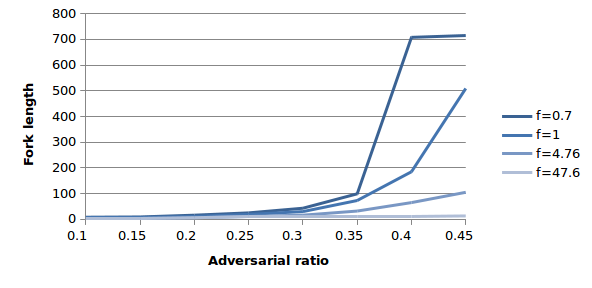
\includegraphics[width=0.75\textwidth]{ghost_split_chart}
        \caption{The fork length that an attacker with a given hashing power could create for the GHOST protocol with the probability of success at least 1\%. Different lines represents different chose of the parameter \(k\).}
        \label{fig:ghost_split_chart}
    \end{figure}
	
	\section{Ouroboros Proof-Of-Stake Protocol}
	
	This section provides the description of the Ouroboros protocol. As stated in \cite{KRDO16} it is the first proof-of-stake blockchain protocol with rigorous security guarantees comparable to those achieved by the Bitcoin blockchain protocol.
	First we will briefly discuss the protocol itself and then look into security guarantees provided by it.
	
	\subsection{General overview}
	
	As were mentioned before, the Ouroboros is a proof-of-stake protocol, thus it does not require heavy computations for block producing. While in the proof-of-work protocols like Bitcoin the blocks are produced by the miners (which are not necessarily have a stake in the system), in Ouroboros only the stakeholders could produce blocks. Given that the stakeholders are well incentivized to keep the overall stability of the system (as it would consequently keep the value of their coins), it creates an additional incentive for block producers to act honestly, thus making a system more secure in general. 
	
	The main idea behind the protocol is that the time is divided into so called epochs, each epoch consists of predefined number of slots. Each slot has an associated stakeholder that should produce a block during the time of that slot. So the model requires a synchrony among stakeholders, the blocks that are produced in the incorrect timeslots are considered invalid. At most one block could be produced in the given slot (Fig. \ref{fig:ouroboros_general}).
	
	The owners of the slots are chosen randomly before each epoch starts. A randomness for a selection procedure is generated collectively by a set of stakeholders via a special cryptographic algorithm based on the PVSS scheme (Publicly Verifiable Secret Sharing \cite{}).
	
	\begin{figure}[h] 
        \centering
        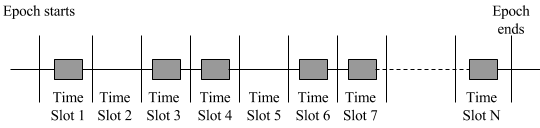
\includegraphics[width=0.75\textwidth]{Ouroboros_general}
        \caption{A general scheme of the Ouroboros protocol. The time is divided on slots, each slot has an associated stakeholder who should produce a block in this slot. It is not necessary that the block in the given slot will produced (for instance, a corresponding stakeholder could be offline at the moment), but there is a strict rule that only one block could be produced in the slot.}
        \label{fig:ouroboros_general}
    \end{figure}
    
    \subsection{The attacks on the common prefix}
    
    Following the terminology given in \cite{KRDO16} the attack that consists in a fork creation is called an attack on a common prefix. There are two possible models for an adversary that is going to create a fork: the one that immediately discovers an adversarial behaviour and the one that leaves an adversary covert. We will briefly describe both of them.
    
    Despite of the rule that a slot winner can produce only one block per slot in the given chain of blocks, nothing can prevent him from creating several blocks in the same slot but on the different chains (see Fig. \ref{fig:ouroboros_split_attack}). By doing this an adversary facilitates an attack forcing the honest slot winners to be split between two chains. In what follows we call such an adversary as "super adversary".
    \begin{figure}[h] 
        \centering
        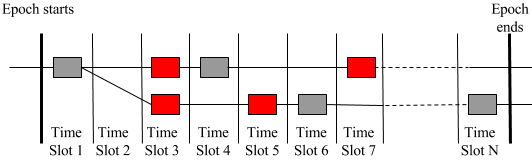
\includegraphics[width=0.75\textwidth]{ouroboros_split_attack}
        \caption{An adversary that possesses some slots (depicted in red) tries to split honest slot winners on two chains, thus facilitating an attack.}
        \label{fig:ouroboros_split_attack}
    \end{figure}
    
    While the described attack provides an adversary significant opportunities it leaves a suspicions "audit trail" - multiple signed blocks at the same slot, which immediately discovers malicious behaviour. This motivates to consider a restricted class of covert adversaries, who produce not more than one block per slot (though not necessarily in the expected slot \cite{KRDO16}).
    
    An interested reader could find more details in \cite{KRDO16, RMKQ17}.
    
    \subsection{Experimental results}
    
    In order to get insights on the density of forks produced by different types of adversaries and to compare them with other consensus protocols, we run several experiments. The results are shown in the Table. \ref{tbl:ouroboros_fork_lengths}.
    
    \myworries{TODO: describe algorithms used for simulation}
    
    Because a synchrony between time slots is assumed in the Ouroboros protocol, it does not make sense to consider the parameter \(k\) as we did for other consensus protocols.
    \begin{table}[h!]
        \label{tbl:ouroboros_fork_lengths}
        \centering
    \begin{tabular}{ | c || c | c | }
         \hline 
         Adversarial stake & Super Adversary & Covert Adversary \\
         \hline
         0.1   & 15  & 9   \\
         0.15  & 23  & 15  \\
         0.2   & 35  & 21  \\
         0.25  & 55  & 33  \\
         0.3   & 94  & 55  \\
         0.35  & 181 & 101 \\
         0.4   & 443 & 235 \\
         0.45  & 1990  & 951 \\
         0.46  & 3214  & 1487 \\
         0.47  & 5953  & 2649 \\
         0.48  & 14157  & 5965 \\
         0.49  & 61922  & 23869 \\
         \hline
    \end{tabular}
    \caption{Fork lengths that an adversary with a given part of the total stake can maintain with the probability at least 0.1\%.}
    \end{table}
	
	\section{Protocols comparison}
	
	This section provides comparison between different consensus protocols described in the previous sections. As a unified measure we took the number of block confirmations (or time slots in case of Ouroboros) needed to be sure that a given block can not be reverted from the blockchain with the probability at least 99.9\% (in other words, the longest fork that an adversary with a certain hashing power/stake can create with the probability of at least 0.1\%). 
	
	The chosen measure appears to be relevant for a real-world application because it shows how long a user should wait to accept a payment transaction, thus decreasing the possibility of the double-spend attack to acceptable level.
	
	The summarized results are presented in Table \ref{tbl:fork_lengths_comparison}. It includes two models for Ouroboros (with super and covert adversary), classic Bitcoin double-spend attack, Bitcoin splitting attack (including hypothetical Bitcoin with reduced block generation time to one per communication round) and GHOST splitting attack.
	
	\myworries{TODO: analyse results from table \ref{tbl:fork_lengths_comparison}. Maybe add some additional charts. It could be helpful to compare protocols not only by number of confirmations but also by waiting time}
	
	\begin{table}[h!]
        \label{tbl:fork_lengths_comparison}
        \centering
    \begin{tabular}{|p{1.6cm}||p{1.5cm}|p{1.5cm}|p{1cm}|p{1cm}|p{1cm}|p{1cm}|p{1.2cm}|p{1.2cm}|}
         \hline 
         Adversarial stake (hashing power) & Ouroboros Super Adversary & Ouroboros Covert Adversary & Bitcoin (Rosenfeld) & Bitcoin (Pinzon) & Bitcoin splitting k=47.6 & Bitcoin splitting k=1 & GHOST splitting k=47.6 & GHOST splitting \(k=1\) \\
         \hline
         0.1   & 15     & 9     & 6     & 5     & 3  & 6  & 3   & 6     \\
         0.15  & 23     & 15    & 9     & 8     & 4  & 7  & 4   & 8     \\
         0.2   & 35     & 21    & 13    & 12    & 4  & 8  & 6   & 11    \\
         0.25  & 55     & 33    & 20    & 19    & 5  & 9  & 9   & 19    \\
         0.3   & 94     & 55    & 32    & 32    & 6  & 10 & 9   & 30    \\
         0.35  & 181    & 101   & 58    & 58    & 8  & 12 & 11  & 73    \\
         0.4   & 443    & 235   & 133   & 134   & 9  & 14 & 12  & 185   \\
         0.45  & 1990   & 951   & 539   & 541   & 14 & 18 & 13  & 509   \\
         0.46  & 3214   & 1487  & 844   & 846   &    &    &     &       \\
         0.47  & 5953   & 2649  & 1502  & 1505  &    &    &     &       \\
         0.48  & 14157  & 5965  & 3382  & 3387  &    &    &     &       \\
         0.49  & 61922  & 23869 & 13533 & 13544 &    &    &     &       \\
         \hline
    \end{tabular}
    \caption{Fork lengths that an adversary with a given part of the total stake (or hashing power in case of proof-of-work) can maintain with the probability at least 0.1\%.}
    \end{table}
	
	\section{Conclusions}
	
	\myworries{TODO}
	
    \printbibliography
	
\end{document}
	
